\subsection{Reimpostazione delle password}
\subsubsection{CanResetPassword}
Per reimpostare la password, il modello \verb|User| deve utilizzare il trait \verb|Illuminate\Auth\Passwords\CanResetPassword|~\cite{LaravelResetPassword}.
\subsubsection{Laravel Route}
Per implementare la reimpostazione delle password sono state definite due route nel file \verb|routes\api\auth.php|:
\begin{lstlisting}[caption={Route per la reimpostazione delle password}, label={lst:route_registration}]
Route::post('forgot-password', [
	PasswordResetLinkController::class, 'store'
]);
Route::post('reset-password', [
	NewPasswordController::class, 'store'
]);
\end{lstlisting}

La prima permette di inviare una e-mail all'utente per reimpostare la propria password, mentre la seconda gestisce la reimpostazione della password.

\subsubsection{Email per reimpostare la password}
L'email che verr\`a inviata all'utente viene definita attraverso una chiusura passata come parametro al metodo \verb|toMailUsing| della classe \verb|Illuminate\Auth\Notifications\ResetPassword| nel metodo \verb|boot()| della classe \verb|App\Providers\AuthServiceProvider|. Tale chiusura \`e definita nel seguente modo:
\begin{lstlisting}[caption={E-mail per reimpostare la password}, label={lst:route_registration}]
ResetPassword::toMailUsing(function ($notifiable, $token) {
	$url = env('APP_AUTH_FRONT') . '/reset-password?token=' . $token;
	
	return (new MailMessage)
		->subject('Reset Password')
		->greeting('Hi, ' . $notifiable->name . '!')
		->line(
			'Someone has requested to change your atARTIST password.
			If you did make this request, click the button below:'
		)
		->action('Reset Password', $url)
		->line(
			'If you didn\`t request this, please ignore this email.'
		);
});
\end{lstlisting}
e produce come risultato l'e-mail nella figura sottostante (Figura~\ref{fig:email_di_psw_reset}).
\begin{figure}[htbp]
	\centering
	\fboxsep=0.5pt
	\fboxrule=0.5pt
	\fcolorbox{black}{black}{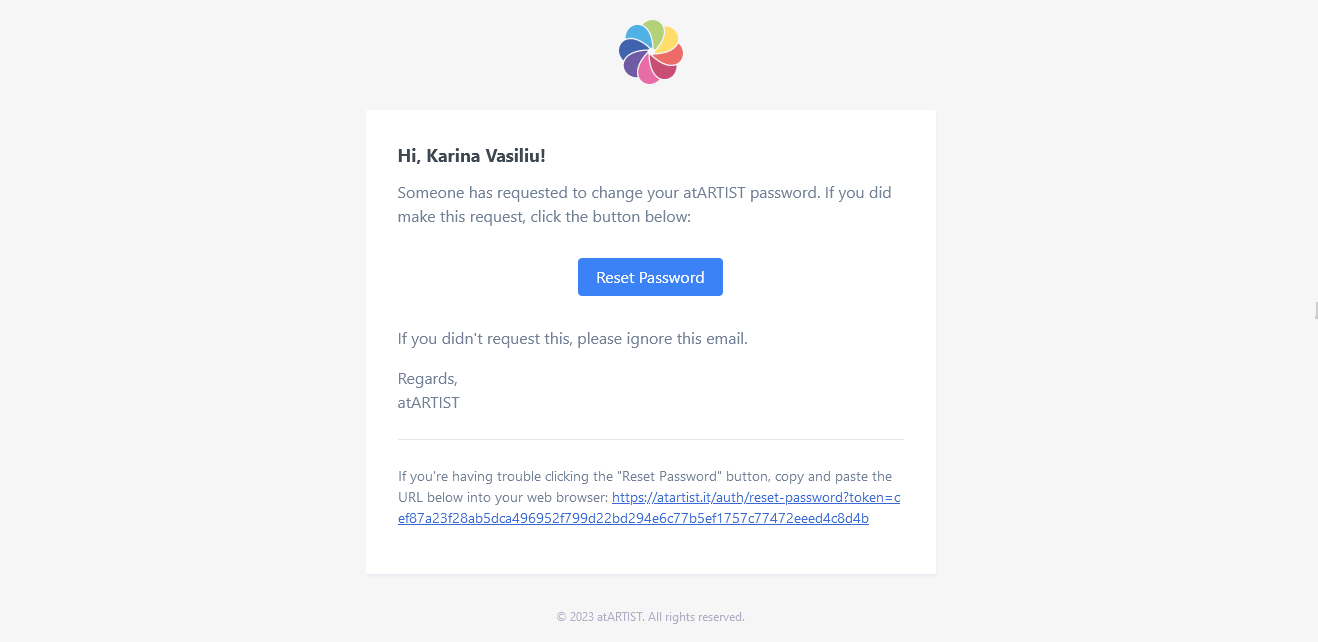
\includegraphics[width=0.8\linewidth]{figure/email_psw}}
	\caption{E-mail per reimpostare la password}
	\label{fig:email_di_psw_reset}
\end{figure}

\subsubsection{Pagina di password dimenticata}
Se durante la fase di accesso l'utente non dovesse ricordare la propria password pu\`o reimpostarla collegandosi alla pagina ``auth/forgot-password'' per compilare il modulo per richiedere di ricevere per email un link per reimpostare la propria password  (Figura~\ref{fig:modulo_reimpostazione_password}). Tale modulo \`e rappresentato dal componente Vue \verb|views\Auth\AuthForgotPassword.vue|:

\begin{figure}[htbp]
	\centering
	\fboxsep=0.5pt
	\fboxrule=0.5pt
	\fcolorbox{black}{black}{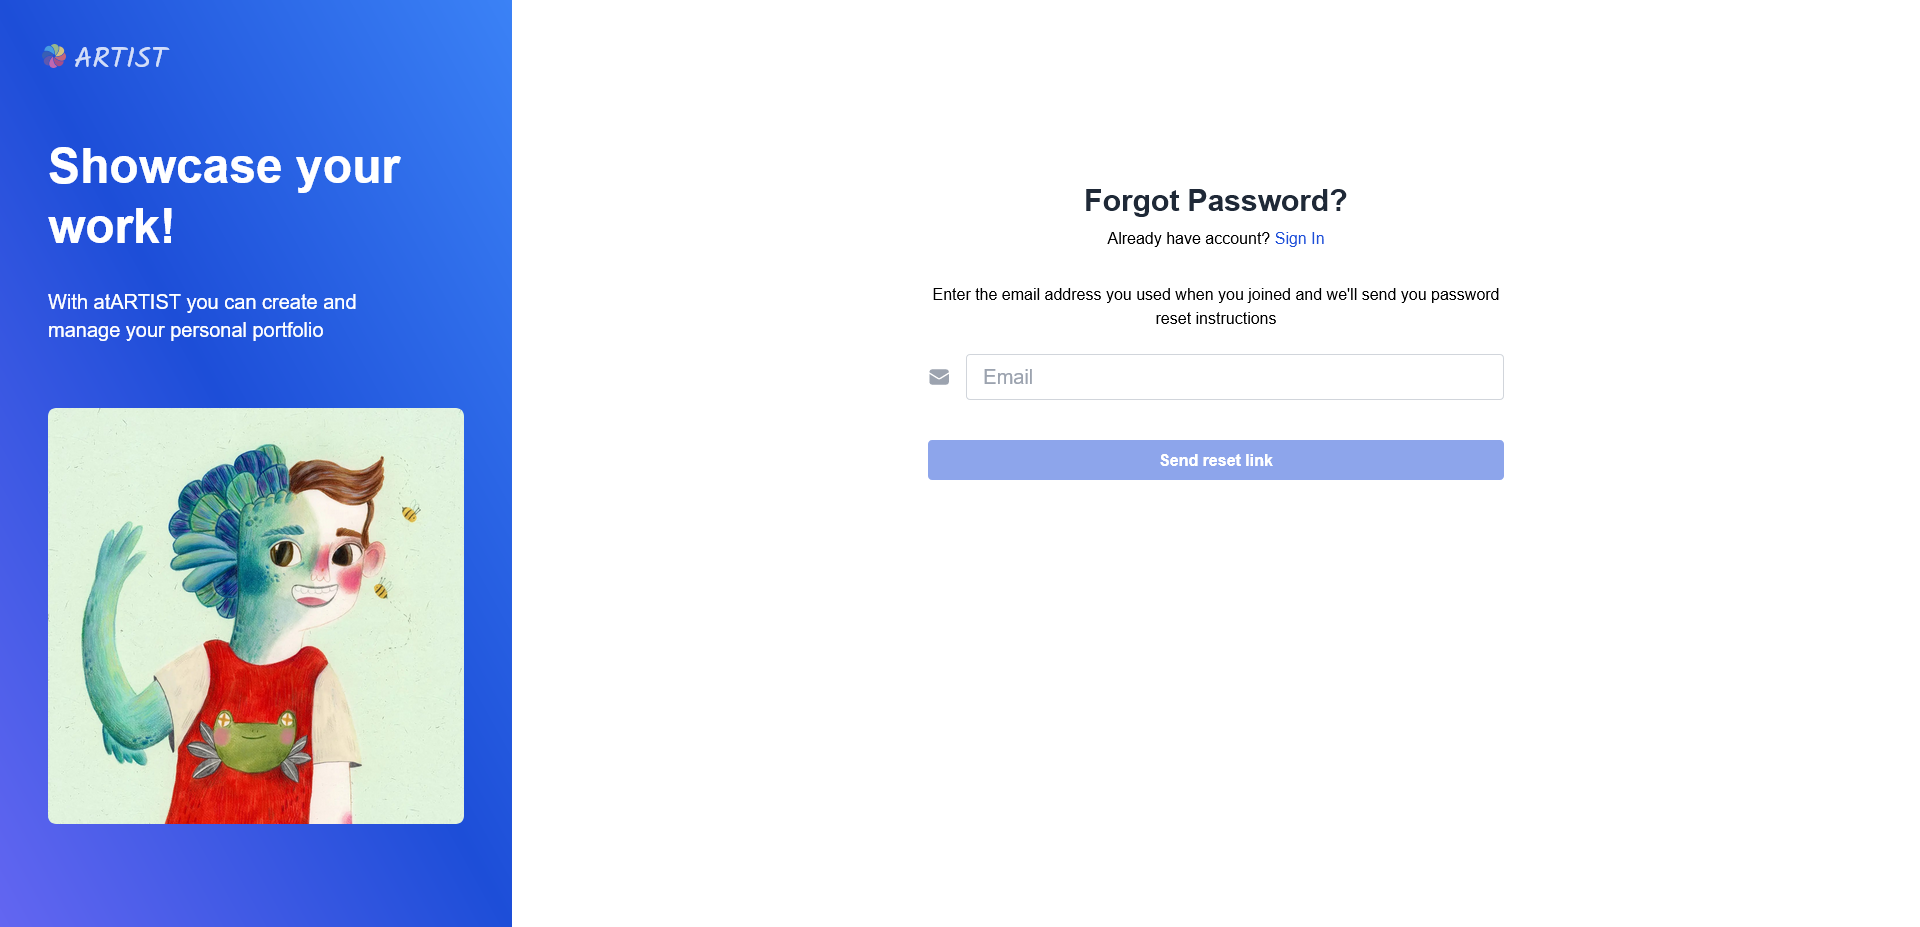
\includegraphics[width=1.0\linewidth]{figure/forget-password}}
	\caption{Pagina di password dimenticata}
	\label{fig:modulo_reimpostazione_password}
\end{figure}

Una volta che l'utente avr\`a compilato il campo e-mail, il modulo potr\`a essere inviato. Sar\`a quindi possibile eseguire la funzione \verb|sendLink| la quale invia una l'e-mail attraverso una richiesta POST all'URI dell'API \verb|auth/forgot-password|. Se l'e-mail non \`e presente nel database viene mostrato un messaggio di errore al di sotto del campo e-mail.

Infine, una volta che il modulo \`e stato compilato ed elaborato correttamente, l'utente verr\`a reindirizzato alla pagina di accesso della piattaforma, nella quale sar\`a presente un messaggio in cima al modulo di accesso che lo avviser\`a del corretto invio della e-mail per la reimpostazione della password.


\subsubsection{Pagina di reimpostazione della password}
Il link ricevuto via e-mail porta l'utente alla pagina ``auth/reset-password'' in modo tale che possa compilare il modulo di reimpostazione della password  (Figura~\ref{fig:modulo_reset_password}).  Tale modulo \`e rappresentato dal componente Vue \verb|views/Auth/AuthResetPassword.vue|. Tale componente, una volta terminato il rendering iniziale, controlla che nell'URL sia presente il parametro \verb|token|, il quale \`e necessario per reimpostare la password.

\begin{figure}[htbp]
	\centering
	\fboxsep=0.5pt
	\fboxrule=0.5pt
	\fcolorbox{black}{black}{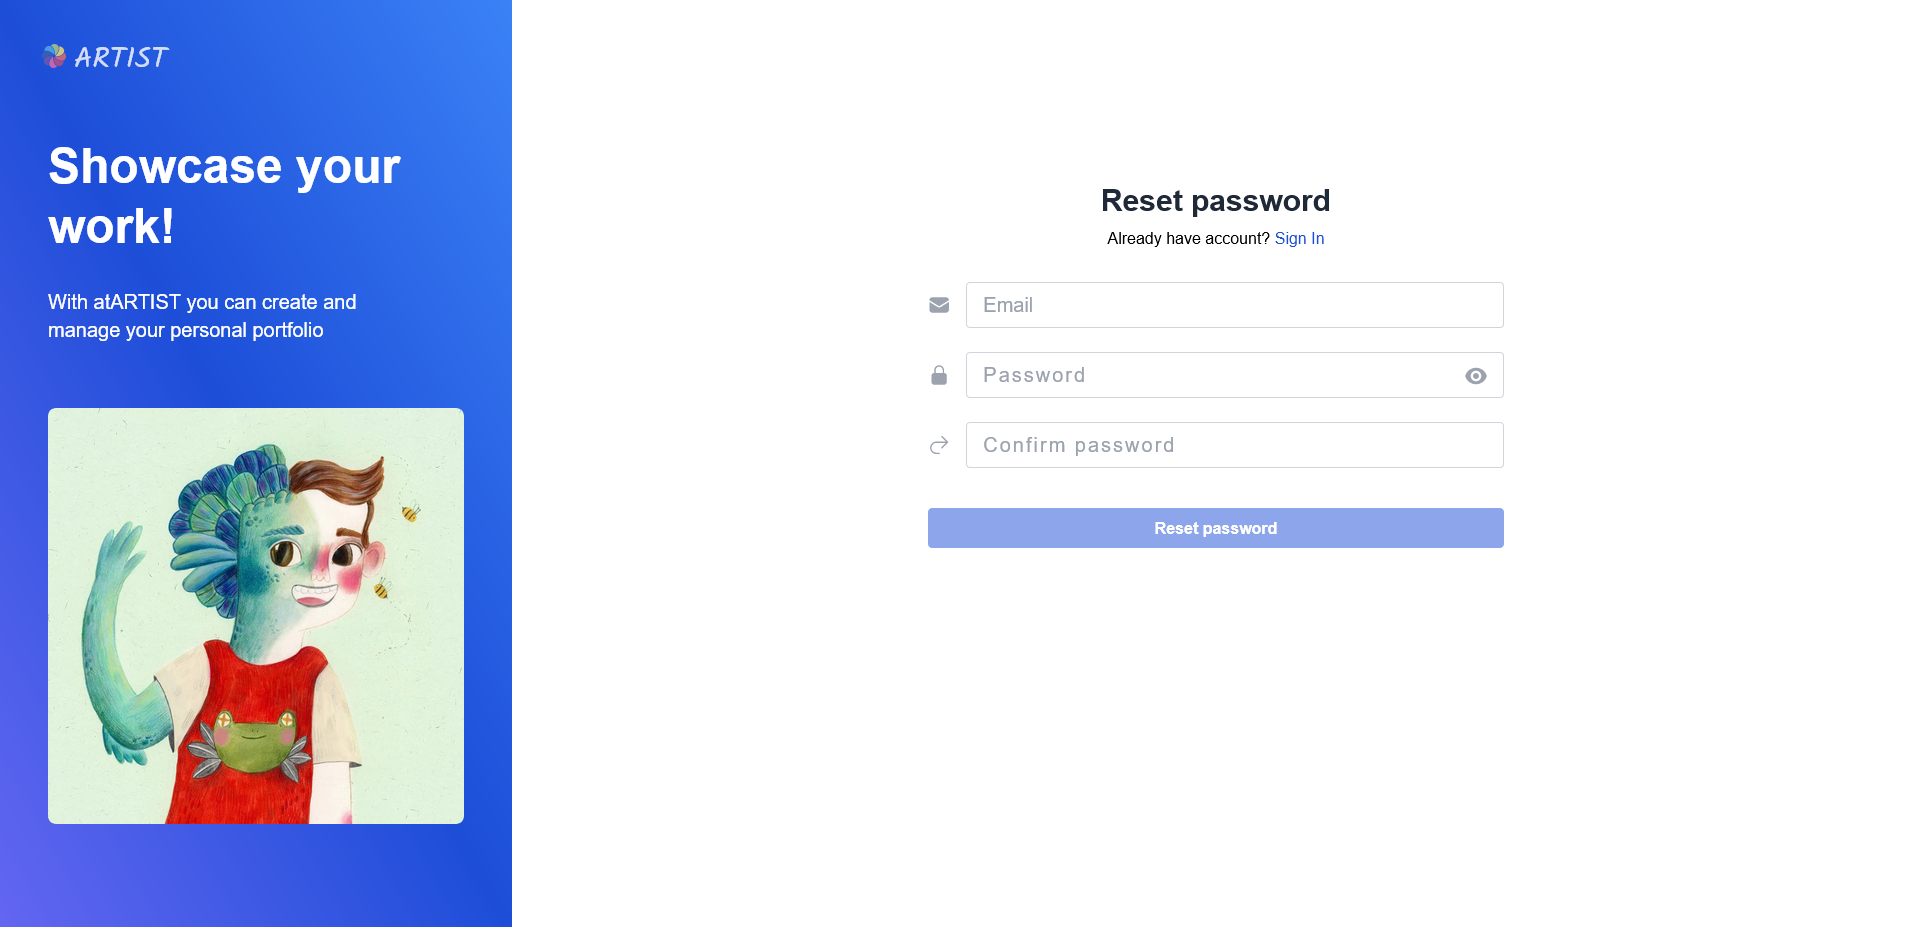
\includegraphics[width=1.0\linewidth]{figure/reset-password}}
	\caption{Pagina di reimpostazione della password}
	\label{fig:modulo_reset_password}
\end{figure}

Una volta che l'utente avr\`a compilato ogni campo, il modulo potr\`a essere inviato. Sar\`a quindi possibile eseguire la funzione \verb|resetPassword| la quale invia i campi del modulo ed il parametro \verb|token| dell'URL attraverso una richiesta POST all'URI dell'API \verb|auth/reset-password|. Se la richiesta fallisce a causa di errori di validazione, vengono mostrati dei messaggi di errore al di sotto dei campi interessati in modo tale che l'utente possa correggerli.

Infine, una volta che il modulo \`e stato compilato ed elaborato correttamente, l'utente verr\`a reindirizzato alla pagina di accesso della piattaforma, nella quale sar\`a presente un messaggio in cima al modulo di accesso che lo avviser\`a della corretta reimpostazione della password.


